\documentclass[11pt,]{article}
\usepackage[left=1in,top=1in,right=1in,bottom=1in]{geometry}
\newcommand*{\authorfont}{\fontfamily{phv}\selectfont}
\usepackage[]{mathpazo}


  \usepackage[T1]{fontenc}
  \usepackage[utf8]{inputenc}



\usepackage{abstract}
\renewcommand{\abstractname}{}    % clear the title
\renewcommand{\absnamepos}{empty} % originally center

\renewenvironment{abstract}
 {{%
    \setlength{\leftmargin}{0mm}
    \setlength{\rightmargin}{\leftmargin}%
  }%
  \relax}
 {\endlist}

\makeatletter
\def\@maketitle{%
  \newpage
%  \null
%  \vskip 2em%
%  \begin{center}%
  \let \footnote \thanks
    {\fontsize{18}{20}\selectfont\raggedright  \setlength{\parindent}{0pt} \@title \par}%
}
%\fi
\makeatother




\setcounter{secnumdepth}{3}

\usepackage{longtable,booktabs}

\usepackage{graphicx,grffile}
\makeatletter
\def\maxwidth{\ifdim\Gin@nat@width>\linewidth\linewidth\else\Gin@nat@width\fi}
\def\maxheight{\ifdim\Gin@nat@height>\textheight\textheight\else\Gin@nat@height\fi}
\makeatother
% Scale images if necessary, so that they will not overflow the page
% margins by default, and it is still possible to overwrite the defaults
% using explicit options in \includegraphics[width, height, ...]{}
\setkeys{Gin}{width=\maxwidth,height=\maxheight,keepaspectratio}

\title{Patrones de distribución, asociación y diversidad de la comunidad de
Chrysobalanaceae utilizando técnicas de ecología numérica en la parcela
permanente de Barro Colorado Island (BCI)  }



\author{\Large Melany Karina Ogando Matos\vspace{0.05in} \newline\normalsize\emph{Estudiante, Universidad Autónoma de Santo Domingo (UASD)}  }


\date{}

\usepackage{titlesec}

\titleformat*{\section}{\normalsize\bfseries}
\titleformat*{\subsection}{\normalsize\itshape}
\titleformat*{\subsubsection}{\normalsize\itshape}
\titleformat*{\paragraph}{\normalsize\itshape}
\titleformat*{\subparagraph}{\normalsize\itshape}

\titlespacing{\section}
{0pt}{36pt}{0pt}
\titlespacing{\subsection}
{0pt}{36pt}{0pt}
\titlespacing{\subsubsection}
{0pt}{36pt}{0pt}





\newtheorem{hypothesis}{Hypothesis}
\usepackage{setspace}

\makeatletter
\@ifpackageloaded{hyperref}{}{%
\ifxetex
  \PassOptionsToPackage{hyphens}{url}\usepackage[setpagesize=false, % page size defined by xetex
              unicode=false, % unicode breaks when used with xetex
              xetex]{hyperref}
\else
  \PassOptionsToPackage{hyphens}{url}\usepackage[unicode=true]{hyperref}
\fi
}

\@ifpackageloaded{color}{
    \PassOptionsToPackage{usenames,dvipsnames}{color}
}{%
    \usepackage[usenames,dvipsnames]{color}
}
\makeatother
\hypersetup{breaklinks=true,
            bookmarks=true,
            pdfauthor={Melany Karina Ogando Matos (Estudiante, Universidad Autónoma de Santo Domingo (UASD))},
             pdfkeywords = {ecología numérica, BCI, Chrysobalanaceae, correlación, agrupamiento,
diversidad},  
            pdftitle={Patrones de distribución, asociación y diversidad de la comunidad de
Chrysobalanaceae utilizando técnicas de ecología numérica en la parcela
permanente de Barro Colorado Island (BCI)},
            colorlinks=true,
            citecolor=blue,
            urlcolor=blue,
            linkcolor=magenta,
            pdfborder={0 0 0}}
\urlstyle{same}  % don't use monospace font for urls

% set default figure placement to htbp
\makeatletter
\def\fps@figure{htbp}
\makeatother

\usepackage{pdflscape} \newcommand{\blandscape}{\begin{landscape}}
\newcommand{\elandscape}{\end{landscape}} \usepackage{float}
\floatplacement{figure}{H}
\newcommand{\beginsupplement}{ \setcounter{table}{0} \renewcommand{\thetable}{S\arabic{table}} \setcounter{figure}{0} \renewcommand{\thefigure}{S\arabic{figure}} }


% add tightlist ----------
\providecommand{\tightlist}{%
\setlength{\itemsep}{0pt}\setlength{\parskip}{0pt}}

\begin{document}
	
% \pagenumbering{arabic}% resets `page` counter to 1 
%
% \maketitle

{% \usefont{T1}{pnc}{m}{n}
\setlength{\parindent}{0pt}
\thispagestyle{plain}
{\fontsize{18}{20}\selectfont\raggedright 
\maketitle  % title \par  

}

{
   \vskip 13.5pt\relax \normalsize\fontsize{11}{12} 
\textbf{\authorfont Melany Karina Ogando Matos} \hskip 15pt \emph{\small Estudiante, Universidad Autónoma de Santo Domingo (UASD)}   

}

}








\begin{abstract}

    \hbox{\vrule height .2pt width 39.14pc}

    \vskip 8.5pt % \small 

\noindent Los patrones de diversidad, distribución y asociación de las especies
con variables ambientales revelan información acerca de como estas
interactúan con el medio ambiente. Utilizando los datos de la
composición de especies de la familia Chrysobalanaceae representadas en
BCI, y mediante diferentes técnicas de ecología númerica, se muestran
los patrones de agrupamiento de los sitios en función de la composición
de especies y su asociación con las variables ambientales, se determinan
las variables ambientales que influyen en la diversidad alpha y cuales
son las especies indicadoras para la diversidad beta. Debido a que los
datos utilizados son datos censales se demostró la completitud de la
muestra por medio de estimadores de riqueza. \emph{Licania }hypoleuca
demostró ser una especie indicadora para uno de los grupos formado por
el análisis de agrupamiento, compuesto por solo 4 sitios. Las variables
ambientales relacionadas a los patrones de agrupamiento son distintas de
aquellas que aportan a la diversidad alpha. Los resultados obtenidos
señalan que las especies poco abundantes son las que caracterizan la
dismilaridad entre sitios cuando estos son cercanos y la variación de
los factores ambientales es leve.


\vskip 8.5pt \noindent \emph{Keywords}: ecología numérica, BCI, Chrysobalanaceae, correlación, agrupamiento,
diversidad \par

    \hbox{\vrule height .2pt width 39.14pc}



\end{abstract}


\vskip 6.5pt


\noindent  \section{Introducción}\label{introducciuxf3n}

Conocer la dispersión y las formas de agrupamiento de los individuos de
una especie, es necesario para su conservación (Condit et al., 1996;
Hubbell \& Foster, 1992). Las especies no son las mismas en todos los
lugares, y estos patrones de variación, en cada uno de los niveles de
diversidad: genes, especies y ecosistemas, es el objeto de estudio de la
biogeografía. Su objetivo es caracterizar la distribución de las
especies en la actualidad y la variación geográfica de la diversidad en
términos de la interacción de los organismos con su ambiente (Lomolino,
Riddle, Whittaker, \& Brown, 2010). La similaridad es una medida simple
de la similitud de especies y sus abundancias. Es convencional decir
que, es lo mismo alta diversidad con alta homogeneidad, lo que es
equivalente a poca dominancia (Magurran, 2004).

Los patrones de biodiversidad son el resultado de la combinación de los
procesos internos de la comunidad de plantas y las condiciones externas
del ambiente (Sang \& Bai, 2008). Por ejemplo, la cantidad de nitrógeno
en el suelo puede ser asumida como una limitante directa en la
distribucion de las especies de plantas (Lange, Nobel, Osmond, \&
Ziegler, 2013). Numerosas especies de la familia Chrysobalanaceae poseen
preferencia por suelos húmedos (Future, 2021; Grandtner \& Chevrette,
2013; Regional Conservation, 2020; C. Sothers, Prance, Buerki, De Kok,
\& Chase, 2014). Esta es una familia de plantas de distribución
pantropical, y cuenta con 18 géneros con 531 especies que se encuentra
un 80\% en el neotrópico (Bardon et al., 2013; G. Prance, 2014).

Las especies de Chrysobalaneceae son utilizadas de maneras distintas
para el tratamiento y como medicina de algunas enfermedades como la
malaria, epilepsia, diarrea y diabetes (Feitosa, Xavier, \& Randau,
2012). Sus usos son frecuentes en la región africana y surámericana,
donde son más abundantes (Feitosa et al., 2012). Posee diferentes usos
como: El aceite de sus frutos para pinturas y varnices, tambien su
madera como material de construcción, combustible y carbón. Además es
utilizada mezclada con arcilla para hacer vasijas de barro (G. Prance,
2014).

La parcela permanente de la isla de Barro Colorado es una reserva de
investigación biológica a cargo del Smithsonian Tropical Research
Institute (Croat, 1978). Según Condit (1998) la distribucion de
\emph{Hirtella americana} en la parcela permanente de BCI se encuentra
de manera irregular en pequeñas áreas isoladas. Sin embargo, los
estudios realizados no han demostrado que esta irregularidad se deba a
variables ambientales. Croat (1978) menciona que \emph{Hirtella
triandra} es una de las especies mayor representadas por su densidad en
este bosque.

En esta investigación se estudia como es la composición de plantas de la
familia Chrysobalanaceae en BCI para descubrir los factores que
intervienen en los modelos de dispersión, diversidad y agrupamiento de
estas especies. El objetivo principal es conocer como estas especies se
relacionan entre ellas y con los factores del ambiente, además de hallar
cuáles son esos factores que contribuyen a los patrones de distribución
espacial de esta familia. Se estima que debido a la cercanía de los
sitios del área de estudio las variables ambientales varían de manera
paulatina, por lo que lo caracterizará cada uno de los sitios es la
presencia de especies raras o poco abundantes, las cuáles deben estar
relacionadas con ciertas variables ambientales.

Se utilizaron distintos técnicas de estudio para conocer como se agrupan
los sitios en función de la composición de especies y cuáles variables
ambientales muestran relación a estos grupos, las especies indicadoras o
con preferencia por algún hábitat, las variables ambientales que
influyen en la diversidad alpha y las especies contribuyentes a la
diversidad beta, y descubrir si los patrones de distribución de las
especies está correlacionado por las variables ambientales.

\section{Metodología}\label{metodologuxeda}

\subsection{Obtención de los datos}\label{obtenciuxf3n-de-los-datos}

Los datos fueron obtenidos del censo realizado durante el 2010 por el
Smithsonian Tropical Research Institute en la parcela permanente de
Barro Colorado Island en el lago Gatún, Panamá (S. Hubbell, Condit, \&
Foster, 2010). En este censo, se contabilizaron todos los árboles con
troncos de al menos 10mm de diámetro de altura de pecho (DAP), y estos
fueron identificados y marcados. Esta parcela cuenta con 50 hectáreas
dividida en 50 cuadros de 1 hectárea cada uno.

\begin{figure}
\centering
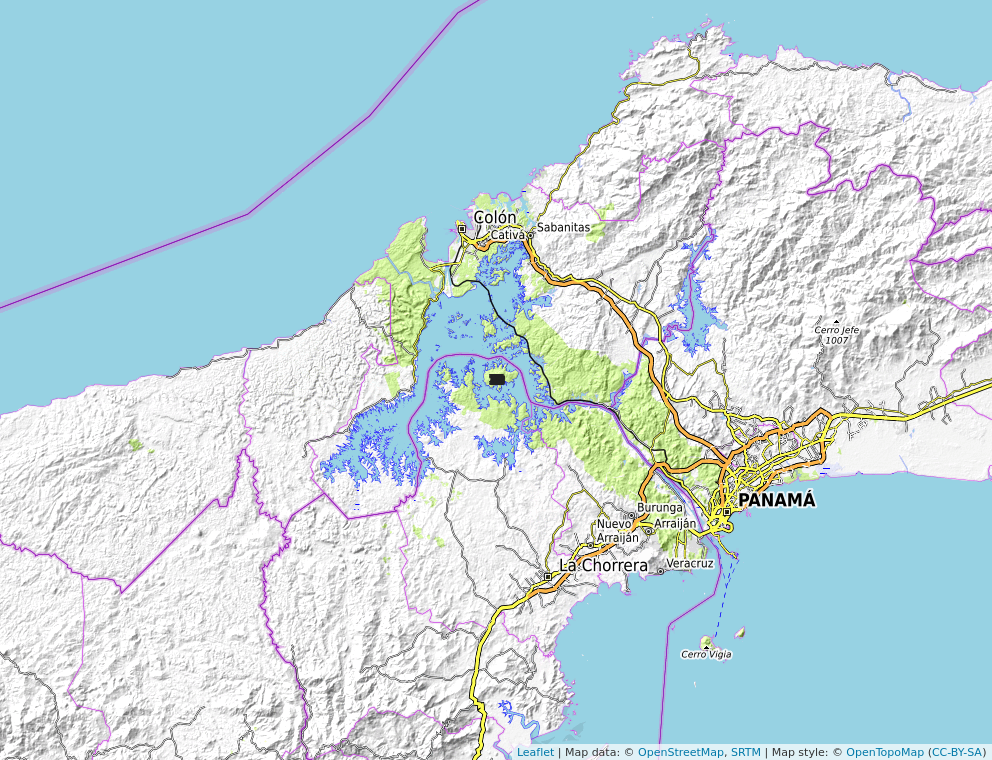
\includegraphics[width=0.50000\textwidth]{mapa_cuadros_panama.png}
\caption{Parcela de 50-ha de Barro Colorado Island,
Panamá\label{mapaBCIcuadros}}
\end{figure}

Los datos utilizados en esta investigación fueron administrados a través
del repositorio Batlle (2020). Estos datos continenen la matriz de
comunidad y la matriz ambiental. En la matriz de comunidad se extrajeron
los datos de la familia Chrysobalanaceae.

\subsection{Análisis estadístico}\label{anuxe1lisis-estaduxedstico}

Para conocer los patrones de agrupamiento según la composición de
especies de Chrysobalanaceae se realizó un análisis de agrupamiento
tomando en consideración cuatro técnicas jerárquicas y aglomerativas
(Borcard, Gillet, Legendre, \& others, 2011; Krebs, 2014), las cuales
fueron: por enlace simple,por enlace completo, por enlace promedio
(UPGMA) y por el método de Ward. Los datos de la matriz de comunidad
fueron normalizados y se calculó la distancia euclídea, para luego
proceder a realizar las técnicas de agrupamiento.

Para conocer el patrón de organización de la familia Chrysobalanaceae y
seleccionar el dendrograma que mejor explica las relaciones entre las
especies de esta familia, se realizaron pruebas de distancia cofenética;
y para conocer el número de grupos óptimos se calculó la anchura de
siluetas. Por medio de Bootstrap multiescalar se revisaron los datos
obtenidos en los métodos anteriores. Para evaluar la relación de los
grupos obtenidos con las variables ambientales se utilizó una prueba de
igualdad de promedios por t student y la prueba no paramétrica de la
suma de rangos de Wilcoxon (medianas). Además, se realizó un análisis de
especies indicadoras mediante la prueba de IndVal y un analisis de
especies con preferencia por hábitat mediante el coeficiente de
correlación biserial puntual (Phi).

Las técnicas de ordenación consisten en colocar objetos o variables en
un espacio donde cada uno representa una dimensión (Borcard et al.,
2011). Los gráficos generados mediante estos análisis muestran una
relación ordenada de las variables formando un diagrama de dispersión
(Legendre \& Gallagher, 2001; Legendre \& Legendre, 2012).

A fin de detectar las tendencias de ordenación de las especies de la
familia Chrysobalanaceae se utilizaron diferentes técnicas de tipo
restringida y no restringida. El análisis de componentes principales
(PCA) se realizó para variables ambientales utilizando solo las
variables numéricas y escalándolas a puntuaciones Z para generar una
matriz de correlaciones; para las variables de la matriz de comunidad
los datos fueron transformados basados en Hellinger. El análisis de
correspondencia (CA) se realizó calculando las distancias de los objetos
en CHI cuadradro. La técnicas de ordenación restringida utilizada fue un
análisis de correspondencia canónica (CCA).

Para el análisis de la diversidad Alpha se calcularon los números de
diversidad Alpha y los ratios de Hill como se encuentra explicado por
Krebs (2014) y Borcard et al. (2011). Los sitios que poseían solo una
especie fueron excluidos. Posteriormente, se realizó un análisis de
correlacion de pearson con las variables ambientales seleccionadas, para
conocer si existe asociación con la diversidad Alpha. Con el objetivo de
medir la diversidad de especies de una localidad cuando solo se tienen
una muestra de la riqueza total de la comunidad, se utilizó el enfoque
asintótico no paramétrico de Chao. La diversidad beta calculada con los
datos de presencia/ausencia de las especies nos dice cúantas más
especies están presentes en toda el área que en un sitio individual
(Borcard et al., 2011). La contribución local de los sitios y las
especies a la diversidad beta fue realizada siguiendo los procedimientos
indicados por Borcard et al. (2011).

Uno de los fundamentos de la ecología espacial es comprender como el
espacio impacta en la estructura de la comunidad (Cantrell, Cosner, \&
Ruan, 2010). La autocorrelación espacial es una medida de la similaridad
o disimilaridad de dos sitios cercanos con relación a los pares
seleccionados aleatoriamente (Borcard et al., 2011). El análisis de
correlacción espacial se realizó siguiendo la metodología descrita por
Batlle (2020). En primer lugar, los datos de la matriz de comunidad
fueron transformados midiendo la distancia Hellinger, y se generó la
vecindad para la matriz ambiental. Entonces, la autocorrelación de las
especies y las variables ambientales se midió a partir de un
correlograma. Posteriormente, se eliminaron las tendencias espaciales de
autocorrelación transformando la matriz de comunidad Hellinger en una
matriz de posiciones XY, para luego realizar una prueba Mantel de
correlograma. De igual forma, se evaluó la autocorrelación espacial por
I de Moran sin tomar en cuenta las tendencias espaciales.

Los análisis fueron realizados en la consola de RStudio (R Core Team,
2020) administrada por José Ramón Martínez Batlle. Para acceder a la
consola se realizó mediante el navegador Google Chrome en una
computadora personal de prestaciones básicas. Los paquetes utilizados
para los diferentes análisis fueron Oksanen et al. (2019), R. Kindt \&
Coe (2005), Wickham (2017) y De Caceres \& Legendre (2009).

\section{Resultados}\label{resultados}

La familia Chrysobalanaceae se encuentra representada en BCI por un
total de 4,821 individuos formada por las especies \emph{Hirtella
americana}, \emph{Hirtella triandra}, \emph{Licania platypus} y
\emph{Licania hypoleuca} \ref{tab:abun_sp}. La especie más abundante fue
\emph{Hirtella triandra}, que representa un 90\% de la composición de la
familia en BCI.

\begin{longtable}[]{@{}lr@{}}
\caption{\label{tab:abun_sp}Tabla de abundancias de las especies de
Chrysobalanaceae en BCI}\tabularnewline
\toprule
Latin & n\tabularnewline
\midrule
\endfirsthead
\toprule
Latin & n\tabularnewline
\midrule
\endhead
Hirtella triandra & 4408\tabularnewline
Licania platypus & 251\tabularnewline
Licania hypoleuca & 141\tabularnewline
Hirtella americana & 21\tabularnewline
\bottomrule
\end{longtable}

Los análisis de agrupamiento por medio de las cuatro técnicas mostraron
grupos similares, con un grupo consistente en todas las técnicas formado
por los sitios 24, 25, 29 y 30. Los dendrogramas que mostraron mayor
correlación cofenética fueron los creados por los métodos de enlace
completo y enlace promedio (UPGMA). El número de grupos obtenido
mediante el cálculo de anchura de silueta fue de dos para los
dendrogramas generados por enlace completo, por enlace pormedio (UPGMA)
y por Ward.

El mapa de calor generado para los dendrogramas muestra ligeramente la
apariencia de tres grupos, sin embargo el análisis mediante boostrap
multiescalar refuerza la partición en solo dos grupos para UPGMA, Ward y
por enlace completo. Ya que los dendrogramas generados por UPGMA y por
enlace completo mostraron resultados muy similares, los dendrogramas
utilizados para posteriores análisis fueron los generados por medio de
agrupamiento por enlace completo y Ward para dos grupos óptimos
\ref{clusters}. El grupo uno formado por 46 sitios y el grupo dos
formado por 4 sitios \ref{mapagrupos}.

\begin{figure}
\centering
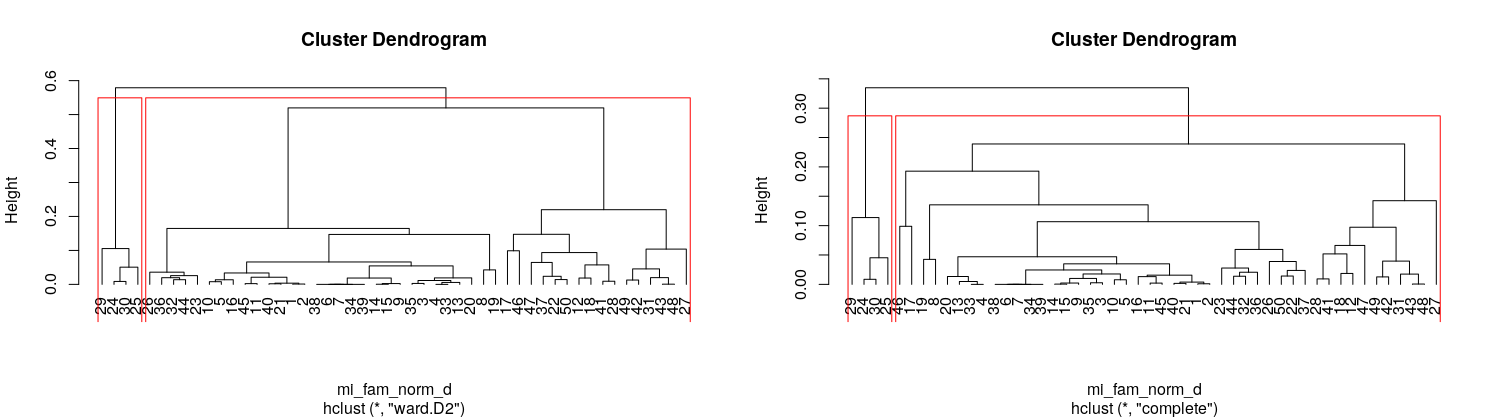
\includegraphics[width=1.00000\textwidth]{Clusters.png}
\caption{Dendrogramas generados por análisis de
agrupamiento\label{clusters}}
\end{figure}

\begin{figure}
\centering
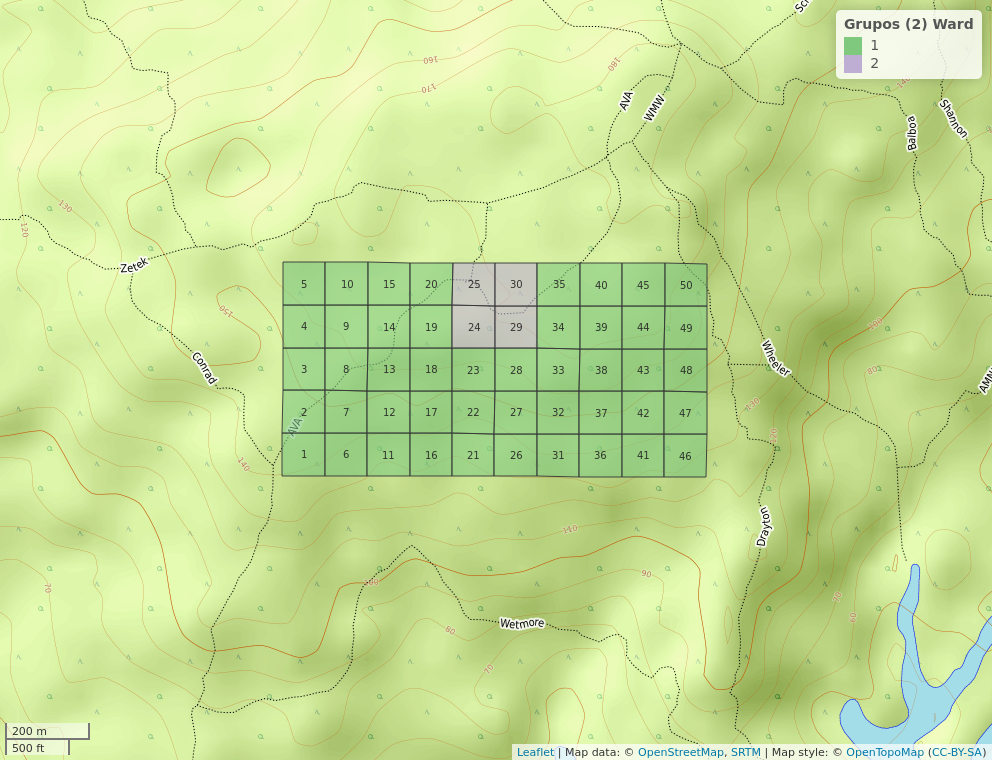
\includegraphics[width=0.50000\textwidth]{mapa_ward_k2.png}
\caption{Mapa según grupos generados por análisis de
agrupamiento\label{mapagrupos}}
\end{figure}

Las pruebas de igualdad de promedios realizadas por medio de t-student
mostró que las variables heterogeneidad ambiental, Nitrógeno y elevación
media muestran relación significativa con los grupos formados por medio
del análisis de agrupamiento. La suma de rangos de Wilcoxon no se
realizó, debido a que esta prueba se utiliza para una anchura de silueta
de tres o más, y los modelos de agrupamiento que se utilizaron se
realizaron para dos grupos óptimos.

Los análisis de especies indicadoras o con preferencia por determinados
hábitats dio como resultado que \emph{Licania hypoleuca} parece ser una
especie indicadora para el grupo 2 (formado por los sitios 24, 25, 29 y
30).

Mediante el cálculo de los factores de inflación (VIF) de las variables
de suelo y ambientales se escogió un grupo reducido de variables que
tuvieran poca correlación entre ellas con un VIF menor de 10. Las
variables escogidos fueron Aluminio, Cobre, Manganeso, Nitrógeno, pH,
Nitrógeno mineralizado, elevación media, heterogeneidad ambiental y
orientación media.

El análisis de componentes principales para los datos de variables
ambientales seleccionadas dio como resultado que los sitios se asocian
en dos grupos distintivos, sin embargo estos grupos no se corresponden
con los generados por medio del análisis de agrupamiento por enlace
completo (\ref{pcagroup}).

\begin{figure}
\centering
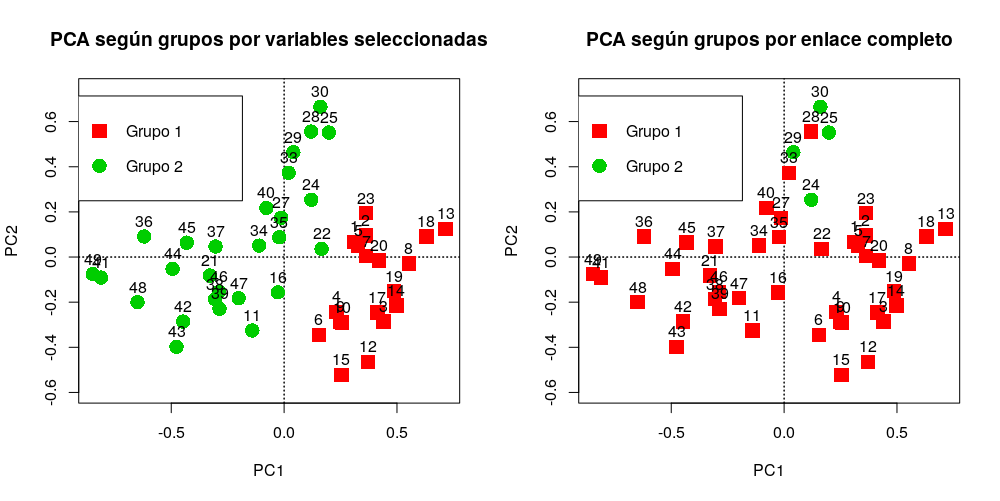
\includegraphics[width=0.80000\textwidth]{PCA_porgrupos.png}
\caption{Analisis de Componentes Principales por grupos\label{pcagroup}}
\end{figure}

El análisis de componentes principales (PCA) aplicado a la matriz de
comunidad muestra la relación de \emph{Licania hypoleuca} con los sitios
del grupo 2 del análisis de agrupamiento generado por enlace completo
\ref{pcaespecies}, al igual que en el análisis de correspondecia. Esta
especie parece asociarse de manera inversa con la abundancia de
Manganeso. Las especies \emph{Hirtella triandra} e \emph{Hirtella
americana} presentan correlación inversa, pues los vectores se muestran
en direcciones completamente opuestas.

\begin{figure}
\centering
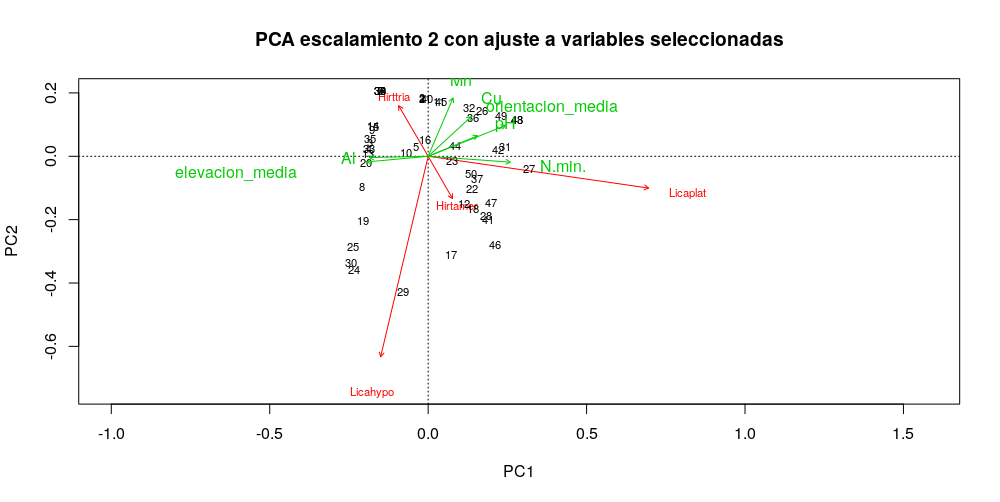
\includegraphics[width=0.80000\textwidth]{PCA_especies.png}
\caption{PCA escalamiento 2 con ajuste a variables
seleccionadas\label{pcaespecies}}
\end{figure}

Los resultados del análisis de correspondencia canónica explican un 47\%
de los datos y en el gráfico se puede verificar que \emph{Hirtella
triandra} es la especie con mayor abundancia, pues se encuentra en el
centro del plano. También se muestra que \emph{Licania platypus} se
encuentra muy correlacionada con la abundancia de nitrógeno mineralizado
(\ref{triplotcca}).

\begin{figure}
\centering
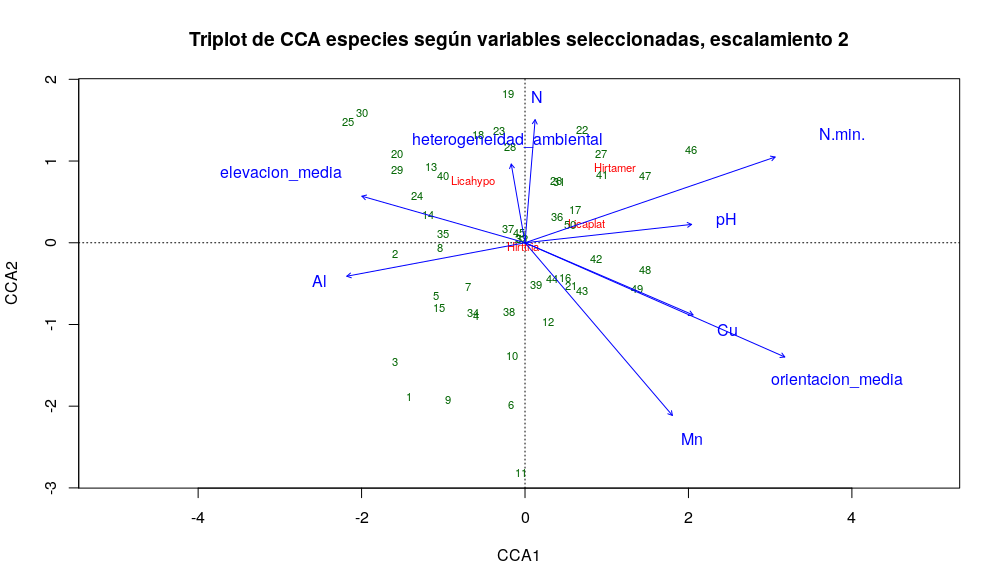
\includegraphics[width=0.80000\textwidth]{triplotCCA.png}
\caption{Triplot de CCA de especies en escalamiento 2\label{triplotcca}}
\end{figure}

Las variables ambientales Magnesio, Zinc, Nitrógeno mineralizado y
geomorfología de interfluvio mostraron relación con los números de Hill.
Mientras que pH y Nitrógeno parecen estar correlacionadas con la equidad
de Pielou (\ref{diversidadalpha}). El trabajo de muestreo realizado en
BCI con relación a la familia Chrysobalanaceae se estima que representa
un 100\% de completitud de la muestra, según los estimadores de Chao
\ref{extrapolacion}, por lo que podemos afirmar que esta familia se
encuentra muy bien representada en BCI.

\begin{figure}
\centering
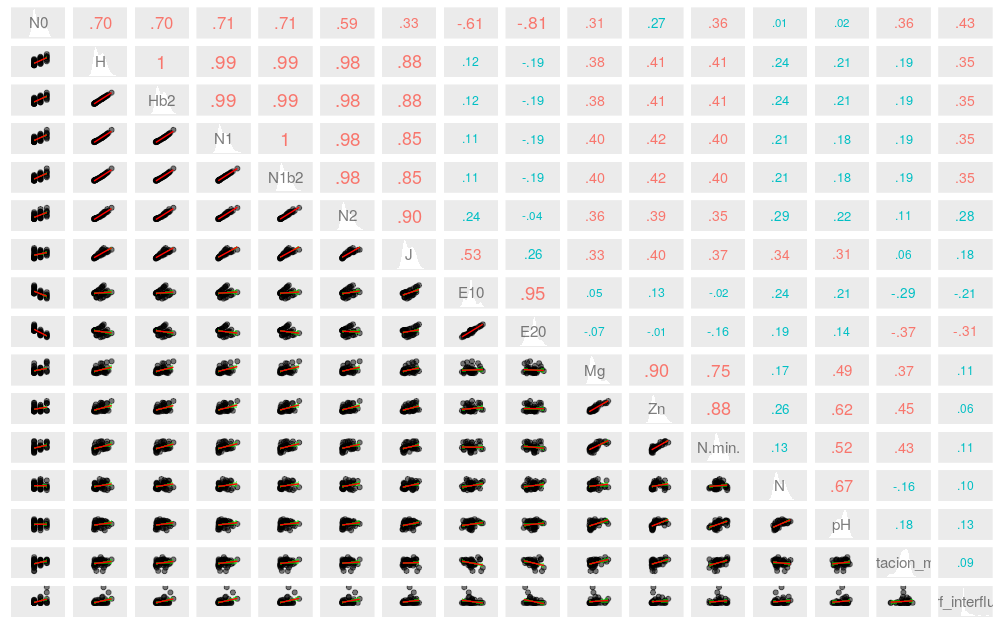
\includegraphics[width=0.80000\textwidth]{diversidadalpha.png}
\caption{Análisis de Correlación de Pearson aplicados a índices de
diversidad según variables ambientales\label{diversidadalpha}}
\end{figure}

\begin{figure}
\centering
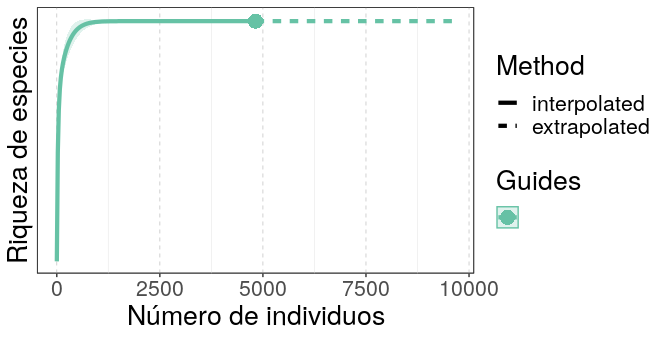
\includegraphics[width=0.80000\textwidth]{Extrapolacion_mifamilia.png}
\caption{Gráfico de rarefacción para toda la
comunidad\label{extrapolacion}}
\end{figure}

Sin embargo, al realizar la estimación de la riqueza por medio de los
estimadores de Chao para los grupos generados en el análisis de
agrupamiento, se estima que el grupo 1 se encuentra representado en un
100\%, pero para el grupo 2 es necesario aumentar el esfuerzo de
muestreo. Esto puede deberse a la desigualdad del número de sitios en
los grupos.

La diversidad beta multiplicativa disminuye mientras aumenta la
importancia de la abundancia más que la riqueza, esto se debe a la
autocorrelación espacial de los sitios, y demuestra que la diversidad de
la comunidad está marcada por la presencia de especies indicadoras. Las
especies que muestran contribución a la diversidad beta son
\emph{Licania hypoleuca} y \emph{Licania platypus}, mientras que ninguno
de los sitios resultó como contribuyente.

Mediante la prueba de correlograma las variables Boro, Calcio, Magnesio,
Zinc, Nitrógeno, pH y Nitrógeno mineralizado mostraron correlación en
múltiples órdenes (\ref{correlograma}). La prueba Mantel sin tendencias
de autocorrelación muestra que en los residuos la correlación no es
significativa, por lo que parece que hay una dependencia espacial
inducida por las variables ambientales. El I de moran aplicado a la
matriz sin tendencia espacial dio como resultado que \emph{Licania
hypoleuca} e \emph{Hirtella triandra} se encuentran en un patrón
aglomerativo (\ref{lisamaps}). La variable que muestra un patrón
aglomerativo común con los grupos generados mediante el análisis de
agrupamiento es la elevación media.

\begin{figure}
\centering
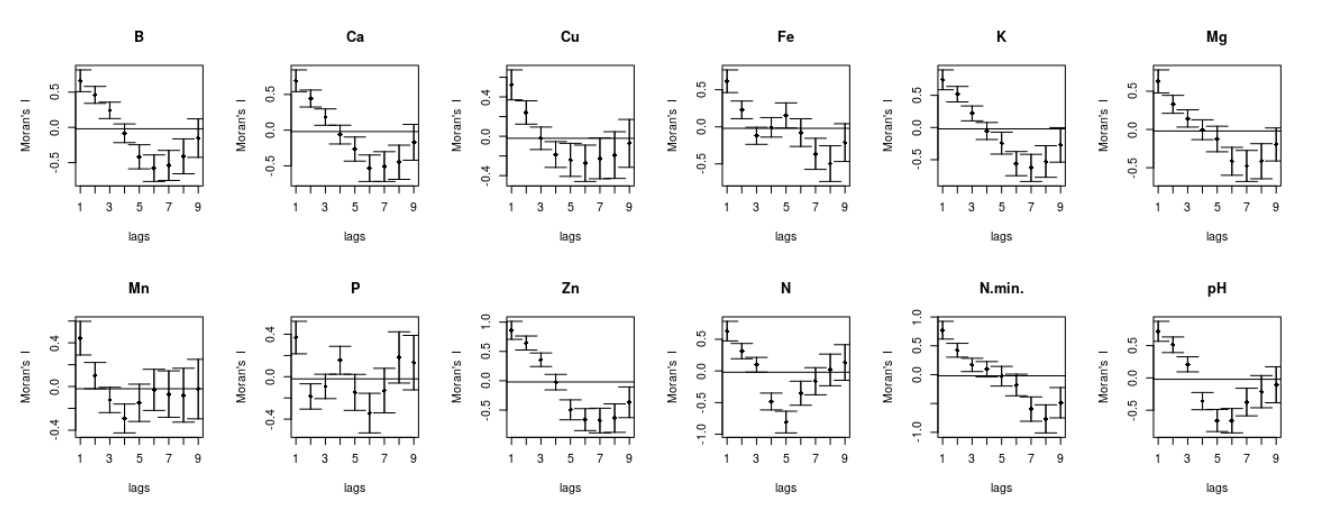
\includegraphics[width=0.80000\textwidth]{correlogramavariables.png}
\caption{Correlograma de variables ambientales\label{correlograma}}
\end{figure}

\begin{figure}
\centering
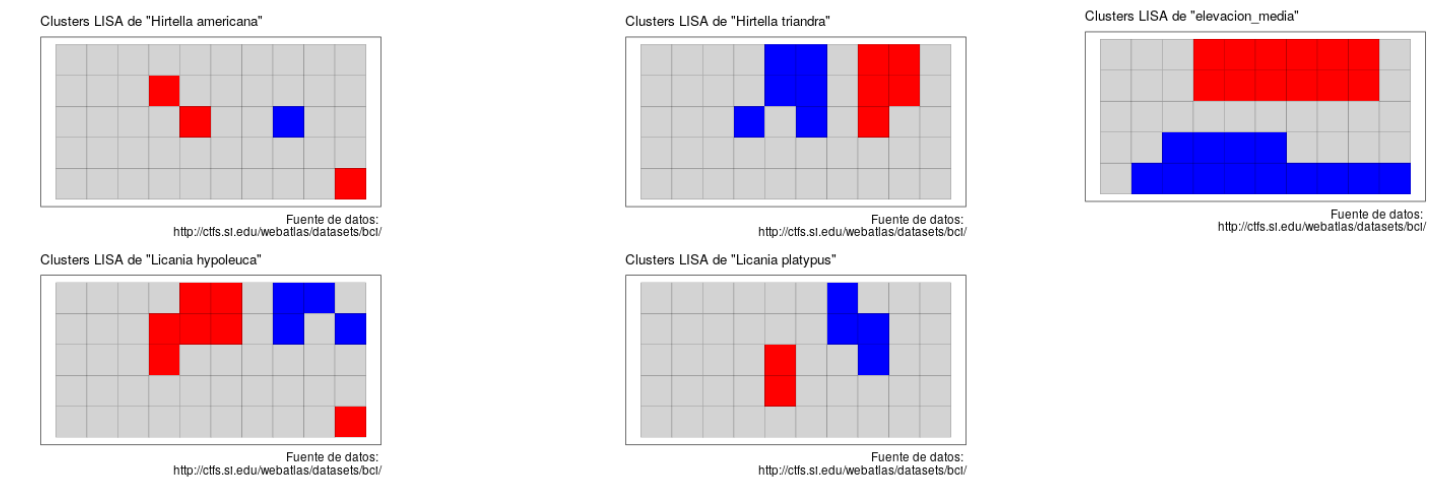
\includegraphics[width=0.80000\textwidth]{clusterlisaespecies.png}
\caption{Mapas Lisa generados para las especies de Chrysobalanaceae y
elvación media\label{lisamaps}}
\end{figure}

\section{Discusión}\label{discusiuxf3n}

La combinación de diferentes técnicas de ecología numérica nos permitió
detectar las relaciones existentes entre la composición de especies de
la familia Chrysobalanaceae y las variables ambientales. Esta familia
posee un alto número de individuos debido a \emph{Hirtella}
\emph{triandra} que es una de las especies más abundantes de BCI. Debido
a que las demás especies pertenecientes a la familia poseen una
abundancia menor de 300 individuos, se confirma que los sitios se
caracterizan por las especies raras.

Los sitios se distinguieron en dos grupos, uno de ellos caracterizado
por la abundancia de \emph{Licania hypoleuca}, este grupo está formado
por los sitios 24, 25, 29 y 30. Las variables ambientales que mostraron
asociación a este grupo fueron la heterogeneidad ambiental, Nitrógeno y
elevación media, las cuáles también se mostraron relacionadas en el
análisis de componentes principales (PCA). Estos hallazagos señalan que
\emph{Licania hypoleuca} es una especie especialista para ambientes con
valores altos de variación de los factores abióticos.

Las técnicas de análisis de ordenación al comparar sitios y especies
muestra que los sitios del grupo 2 se encuentran correlacionados con la
abundancia de \emph{Licania hypoleuca}, y esta a su vez parece asociarse
de manera inversa con la abundancia de Manganeso. Estos resultados
confirman la hipótesis de que los sitios se caracterizan por la
presencia de la especies raras, y la abundancia de estas especies está
determinada por las variables ambientales. El análisis de correspondecia
canónica señala que \emph{Hirtella triandra} e \emph{Hirtella americana}
se relacionan de manera inversa. Esto se refleja en los sitios donde
\emph{H. americana} es más abundante, los cuáles son los sitios donde
\emph{H. triandra} tiene un menor número de individuos. Esto puede
significar que la distribución de \emph{H. americana} no es de manera
irregular, como explica Condit (1998), sino que es inversamente
proporcional a la abundancia de \emph{H. triandra}.

Las varibles ambientales que mostraron relación con el agrupamiento de
los sitios no fueron las mismas que se relacionan con la diversidad
alpha, estos resultados no confirman la premisa de que los factores
ambientales que influyen en la diversidad alpha son los mismos que
determinan la composición de especies en el agrupamiento de los sitios.
El método de muestreo utilizado para generar la base de datos usada en
esta investigación se trata de un censo, por lo tanto se espera que el
análisis de estimación de riqueza muestra una alta completitud de la
muestra, y estos son los resultados que se obtiene al realizar los
estimadores de riqueza de Chao.

Las especies \emph{Licania hypoleuca} e \emph{Licania platypus} son las
especies que resultaron contribuyentes a la diversidad beta de la
comunidad, este resultado confirma lo obtenido en el estudio de especies
indicadoras en el análisis de agrupamiento, pero aporta nueva
información mostrando a \emph{L. platypus} como una especie que aporta a
la variación de la diversidad entre sitios, esto puede deberse a la poca
abundancia que posee en comparación a la abundancia total de la familia.

Los datos parecen mostrar una correlación espacial inducida por algunas
variables ambientales esto confirma que, la cercanía de los sitios
aumenta la correlación espacial debido a que la variación de los
facotres abióticos en zonas cercanas son bajos. Al generar los mapas
Lisa las especies \emph{Licania hypoleuca} e \emph{Hirtella triandra}
parecen mostrar un patrón aglomerado y se solapan con los sitios del
grupo 2, lo cual demuestra que los valores de abundancia altos de
\emph{Licania hypoleuca} son una de las caracteristicas de este grupo, y
además modela que se relaciona con una baja abundancia de \emph{Hirtella
triandra}. La orientación media también muestra un patrón aglomerado que
solapa con los sitios del grupo 2, confirmando una vez más que esta
variable es una de las características de estos sitios.

El hallazgo de que las especies poco abundantes son las que caracterizan
los sitios, y estás a su vez son dependendientes de diversos factores
ambientales, implica que los patrones diversidad, distribución y
asociación de las comunidades son determinados por las especies
especialistas. Posterior a estos estudios, se recomienda aplicar
técnicas de ecología numérica a diferentes grupos de datos para comparar
los resultados, y abundar en como las especies son una característica
importante para la descripción de los hábitat, y a su vez como estas se
relacionan o son dependientes de diferentes variables ambientales.
También es posible realizar nuevos estudios de esta familia pero en
sitios distintos para identificar como estás especies interactúan unas
con otras y con las variables del ambiente.

\section{Agradecimientos}\label{agradecimientos}

Agradezco al profesor José Martínez Batlle por sus enseñanzas y su apoyo
en el análisis de esta investigación. También al Smithsonian Tropical
Research Institute por la obtención y el suministro de los datos.

\section{\texorpdfstring{\emph{Script}
reproducible}{Script reproducible}}\label{script-reproducible}

\begin{verbatim}
##   [1] "#' Script Reproducible"                                                                                                                                                
##   [2] "#' "                                                                                                                                                                   
##   [3] "#' "                                                                                                                                                                   
##   [4] "#' Cargar paquetes"                                                                                                                                                    
##   [5] "#'"                                                                                                                                                                    
##   [6] "library(vegan)"                                                                                                                                                        
##   [7] "library(tidyverse)"                                                                                                                                                    
##   [8] "library(sf)"                                                                                                                                                           
##   [9] "source('biodata/funciones.R')"                                                                                                                                         
##  [10] "#'"                                                                                                                                                                    
##  [11] "#' Cargar datos"                                                                                                                                                       
##  [12] "load('biodata/Chrysobalanaceae.Rdata')"                                                                                                                                
##  [13] "load('biodata/matriz_ambiental.Rdata')"                                                                                                                                
##  [14] "bci_env_grid %>% tibble"                                                                                                                                               
##  [15] "censo_chrys %>% tibble"                                                                                                                                                
##  [16] "#'"                                                                                                                                                                    
##  [17] "#' Analisis Exploratorio"                                                                                                                                              
##  [18] "#' Lista de especies: 4"                                                                                                                                               
##  [19] "sort(colnames(mc_chrys))"                                                                                                                                              
##  [20] "#'"                                                                                                                                                                    
##  [21] "#' Abundancia de toda la comunidad"                                                                                                                                    
##  [22] "sum(colSums(mc_chrys))"                                                                                                                                                
##  [23] "#'"                                                                                                                                                                    
##  [24] "#' Abundancia por cuadrante"                                                                                                                                           
##  [25] "sort(rowSums(mc_chrys))"                                                                                                                                               
##  [26] "#'"                                                                                                                                                                    
##  [27] "#' Abundancia por especie"                                                                                                                                             
##  [28] "sort(colSums(mc_chrys))"                                                                                                                                               
##  [29] "#'"                                                                                                                                                                    
##  [30] "#' Tabla de abundancias"                                                                                                                                               
##  [31] "abun_sp <- censo_chrys %>%"                                                                                                                                            
##  [32] "  group_by(Latin) %>% "                                                                                                                                                
##  [33] "  count() %>% "                                                                                                                                                        
##  [34] "  arrange(desc(n))"                                                                                                                                                    
##  [35] "abun_sp"                                                                                                                                                               
##  [36] "#'"                                                                                                                                                                    
##  [37] "#' Analisis de Agrupamiento"                                                                                                                                           
##  [38] "#' Cargar otros paquetes"                                                                                                                                              
##  [39] "library(cluster)"                                                                                                                                                      
##  [40] "library(gclus)"                                                                                                                                                        
##  [41] "library(pvclust)"                                                                                                                                                      
##  [42] "library(mapview)"                                                                                                                                                      
##  [43] "library(RColorBrewer)"                                                                                                                                                 
##  [44] "library(broom)"                                                                                                                                                        
##  [45] "library(indicspecies)"                                                                                                                                                 
##  [46] "#'"                                                                                                                                                                    
##  [47] "#' Crear abreviaturas de la familia"                                                                                                                                   
##  [48] "mi_fam <- mc_chrys"                                                                                                                                                    
##  [49] "(colnames(mi_fam) <- make.cepnames(colnames(mi_fam)))"                                                                                                                 
##  [50] "(df_equivalencias <- data.frame("                                                                                                                                      
##  [51] "  nombre_original = colnames(mc_chrys),"                                                                                                                               
##  [52] "  colnames(mi_fam)))"                                                                                                                                                  
##  [53] "#'"                                                                                                                                                                    
##  [54] "grupos_ward_k2 <- readRDS('grupos_ward_k2.RDS')"                                                                                                                       
##  [55] "table(grupos_ward_k2)"                                                                                                                                                 
##  [56] "grupos_compl_k2 <- readRDS('grupos_compl_k2.RDS')"                                                                                                                     
##  [57] "table(grupos_compl_k2)"                                                                                                                                                
##  [58] "#'"                                                                                                                                                                    
##  [59] "#'#' Cargar paletas de colores"                                                                                                                                        
##  [60] "rojo <- colorRampPalette(brewer.pal(8, \"Reds\"))"                                                                                                                     
##  [61] "rojo_inv <- colorRampPalette(rev(brewer.pal(8, \"Reds\")))"                                                                                                            
##  [62] "colores_grupos <- brewer.pal(8, \"Accent\")"                                                                                                                           
##  [63] "#'"                                                                                                                                                                    
##  [64] "#' Transformar la matriz de comunidad"                                                                                                                                 
##  [65] "#'"                                                                                                                                                                    
##  [66] "mi_fam_norm <- decostand(mi_fam, \"normalize\")"                                                                                                                       
##  [67] "mi_fam_norm_d <- vegdist(mi_fam_norm, \"euc\")"                                                                                                                        
##  [68] "mi_fam_norm_d %>% tidy"                                                                                                                                                
##  [69] "attr(mi_fam_norm_d, \"labels\") <- rownames(mi_fam)"                                                                                                                   
##  [70] "#' "                                                                                                                                                                   
##  [71] "#' Agrupamiento por Enlace completo"                                                                                                                                   
##  [72] "(cl_complete <- hclust(mi_fam_norm_d, method = 'complete'))"                                                                                                           
##  [73] "plot(cl_complete, labels = rownames(mi_fam), hang = -1,"                                                                                                               
##  [74] "     main = \"Sitios de BCI según composición de especies de Chrysobalanaceae\\nEnlace completo a partir de matriz de distancia de cuerdas\","                         
##  [75] "     xlab = 'Sitios', ylab = 'Altura')"                                                                                                                                
##  [76] "#' Agrupamiento por medio de Ward"                                                                                                                                     
##  [77] "(cl_ward <- hclust(mi_fam_norm_d, method = 'ward.D2'))"                                                                                                                
##  [78] "plot(cl_ward, labels = rownames(mi_fam), hang = -1,"                                                                                                                   
##  [79] "     main = \"Sitios de BCI según composición de especies de Chrysobalanaceae\\nMétodo de Ward a partir de matriz de distancia de cuerdas\","                          
##  [80] "     xlab = 'Sitios', ylab = 'Altura')"                                                                                                                                
##  [81] "#' "                                                                                                                                                                   
##  [82] "#' Medicion de la correlacion cofenetica"                                                                                                                              
##  [83] "#' "                                                                                                                                                                   
##  [84] "lista_cl <- list("                                                                                                                                                     
##  [85] "  cl_complete = hclust(mi_fam_norm_d, method = 'complete'),"                                                                                                           
##  [86] "  cl_ward = hclust(mi_fam_norm_d, method = 'ward.D2')"                                                                                                                 
##  [87] ")"                                                                                                                                                                     
##  [88] "par(mfrow = c(1,2))"                                                                                                                                                   
##  [89] "invisible(map(names(lista_cl), function(x) plot(lista_cl[[x]], main = x, hang = -1, cex.lab = 1)))"                                                                    
##  [90] "par(mfrow = c(1,1))"                                                                                                                                                   
##  [91] "#'"                                                                                                                                                                    
##  [92] "map_df(lista_cl, function(x) {"                                                                                                                                        
##  [93] "  coph_d <- cophenetic(x)"                                                                                                                                             
##  [94] "  corr <- cor(mi_fam_norm_d, coph_d)"                                                                                                                                  
##  [95] "  return(corr)"                                                                                                                                                        
##  [96] "})"                                                                                                                                                                    
##  [97] "#'"                                                                                                                                                                    
##  [98] "#' Calculo de la anchura de siluetas"                                                                                                                                  
##  [99] "#'"                                                                                                                                                                    
## [100] "anch_sil_ward <- calcular_anchuras_siluetas("                                                                                                                          
## [101] "  mc_orig = mi_fam, "                                                                                                                                                  
## [102] "  distancias = mi_fam_norm_d, "                                                                                                                                        
## [103] "  cluster = lista_cl$cl_ward)"                                                                                                                                         
## [104] "anch_sil_ward"                                                                                                                                                         
## [105] "w_dend_reord <- reorder.hclust(lista_cl$cl_ward, mi_fam_norm_d)"                                                                                                       
## [106] "plot(w_dend_reord, hang = -1)"                                                                                                                                         
## [107] "rect.hclust("                                                                                                                                                          
## [108] "  tree = w_dend_reord,"                                                                                                                                                
## [109] "  k = anch_sil_ward$n_grupos_optimo)"                                                                                                                                  
## [110] "heatmap("                                                                                                                                                              
## [111] "  as.matrix(mi_fam_norm_d),"                                                                                                                                           
## [112] "  Rowv = as.dendrogram(w_dend_reord),"                                                                                                                                 
## [113] "  symm = TRUE,"                                                                                                                                                        
## [114] "  margin = c(3, 3),"                                                                                                                                                   
## [115] "  col = rev(cm.colors(4))"                                                                                                                                             
## [116] ")"                                                                                                                                                                     
## [117] "#' Bootstrap"                                                                                                                                                          
## [118] "cl_pvclust_ward <-"                                                                                                                                                    
## [119] "  pvclust(t(mi_fam_norm),"                                                                                                                                             
## [120] "          method.hclust = \"ward.D2\","                                                                                                                                
## [121] "          method.dist = \"euc\","                                                                                                                                      
## [122] "          iseed = 191, # Resultado reproducible"                                                                                                                       
## [123] "          parallel = TRUE)"                                                                                                                                            
## [124] "plot(cl_pvclust_ward, hang = -1)"                                                                                                                                      
## [125] "lines(cl_pvclust_ward)"                                                                                                                                                
## [126] "pvrect(cl_pvclust_ward, alpha = 0.91, border = 4)"                                                                                                                     
## [127] "saveRDS(grupos_ward_k2, 'grupos_ward_k2.RDS')"                                                                                                                         
## [128] "#' Para complete"                                                                                                                                                      
## [129] "anch_sil_compl <- calcular_anchuras_siluetas("                                                                                                                         
## [130] "  mc_orig = mi_fam, "                                                                                                                                                  
## [131] "  distancias = mi_fam_norm_d, "                                                                                                                                        
## [132] "  cluster = lista_cl$cl_complete)"                                                                                                                                     
## [133] "anch_sil_compl"                                                                                                                                                        
## [134] "(grupos_compl_k2 <- as.factor(cutree(lista_cl$cl_complete, k = 2)))"                                                                                                   
## [135] "table(grupos_compl_k2)"                                                                                                                                                
## [136] "#'"                                                                                                                                                                    
## [137] "w_dend_reord <- reorder.hclust(lista_cl$cl_complete, mi_fam_norm_d)"                                                                                                   
## [138] "plot(w_dend_reord, hang = -1)"                                                                                                                                         
## [139] "rect.hclust("                                                                                                                                                          
## [140] "  tree = w_dend_reord,"                                                                                                                                                
## [141] "  k = anch_sil_compl$n_grupos_optimo)"                                                                                                                                 
## [142] "#'"                                                                                                                                                                    
## [143] "heatmap("                                                                                                                                                              
## [144] "  as.matrix(mi_fam_norm_d),"                                                                                                                                           
## [145] "  Rowv = as.dendrogram(w_dend_reord),"                                                                                                                                 
## [146] "  symm = TRUE,"                                                                                                                                                        
## [147] "  margin = c(3, 3),"                                                                                                                                                   
## [148] "  col = rev(cm.colors(4))"                                                                                                                                             
## [149] ")"                                                                                                                                                                     
## [150] "#' Bootstrap"                                                                                                                                                          
## [151] "cl_pvclust_compl <-"                                                                                                                                                   
## [152] "  pvclust(t(mi_fam_norm),"                                                                                                                                             
## [153] "          method.hclust = \"complete\","                                                                                                                               
## [154] "          method.dist = \"euc\","                                                                                                                                      
## [155] "          iseed = 27, # Resultado reproducible"                                                                                                                        
## [156] "          parallel = TRUE)"                                                                                                                                            
## [157] "plot(cl_pvclust_compl, hang = -1)"                                                                                                                                     
## [158] "lines(cl_pvclust_compl)"                                                                                                                                               
## [159] "pvrect(cl_pvclust_compl, alpha = 0.91, border = 4)"                                                                                                                    
## [160] "(grupos_compl_k2 <- as.factor(cutree(lista_cl$cl_complete, k = 2)))"                                                                                                   
## [161] "table(grupos_compl_k2)"                                                                                                                                                
## [162] "saveRDS(grupos_compl_k2, 'grupos_compl_k2.RDS')"                                                                                                                       
## [163] "#'"                                                                                                                                                                    
## [164] "#' Relación de Variables ambientales con grupos de Ward"                                                                                                               
## [165] "(m_amb_ward_k2 <- bci_env_grid %>%"                                                                                                                                    
## [166] "    select_if(is.numeric) %>% select(-id) %>% "                                                                                                                        
## [167] "    mutate(grupos_ward_k2) %>%"                                                                                                                                        
## [168] "    st_drop_geometry() %>% "                                                                                                                                           
## [169] "    pivot_longer(-grupos_ward_k2, names_to = \"variable\", values_to = \"valor\"))"                                                                                    
## [170] "#' "                                                                                                                                                                   
## [171] "m_amb_ward_k2 %>%"                                                                                                                                                     
## [172] "  group_by(variable) %>%"                                                                                                                                              
## [173] "  summarise("                                                                                                                                                          
## [174] "    p_valor_t = t.test(valor ~ grupos_ward_k2)$p.value,"                                                                                                               
## [175] "    p_valor_w = wilcox.test(valor ~ grupos_ward_k2, exact = F)$p.value) %>%"                                                                                           
## [176] "  arrange(p_valor_t) %>%"                                                                                                                                              
## [177] "  print(n=Inf)"                                                                                                                                                        
## [178] "#' "                                                                                                                                                                   
## [179] "m_amb_ward_k2 %>% "                                                                                                                                                    
## [180] "  group_by(variable) %>% "                                                                                                                                             
## [181] "  ggplot() + aes(x = grupos_ward_k2, y = valor, fill = grupos_ward_k2) + "                                                                                             
## [182] "  geom_boxplot() + "                                                                                                                                                   
## [183] "  scale_fill_brewer(palette = 'Accent') +"                                                                                                                             
## [184] "  theme_bw() +"                                                                                                                                                        
## [185] "  theme(legend.position=\"none\") +"                                                                                                                                   
## [186] "  facet_wrap(~ variable, scales = 'free_y')"                                                                                                                           
## [187] "#' "                                                                                                                                                                   
## [188] "#' Mapa de grupos por medio de Ward"                                                                                                                                   
## [189] "mapa_ward_k2 <- mapView("                                                                                                                                              
## [190] "  bci_env_grid %>% mutate(grupos_ward_k2),"                                                                                                                            
## [191] "  layer.name = 'Grupos (2) Ward',"                                                                                                                                     
## [192] "  alpha.regions = 0.6,"                                                                                                                                                
## [193] "  map.types = 'OpenTopoMap',"                                                                                                                                          
## [194] "  legend = T,"                                                                                                                                                         
## [195] "  col.regions = colores_grupos[1:2],"                                                                                                                                  
## [196] "  zcol = 'grupos_ward_k2') %>%"                                                                                                                                        
## [197] "  addStaticLabels(label = bci_env_grid$id) %>% "                                                                                                                       
## [198] "  leaflet::setView("                                                                                                                                                   
## [199] "    lng = -79.85136,"                                                                                                                                                  
## [200] "    lat = 9.15097,"                                                                                                                                                    
## [201] "    zoom = 16)"                                                                                                                                                        
## [202] "mapa_ward_k2"                                                                                                                                                          
## [203] "#' "                                                                                                                                                                   
## [204] "#' Especies indicadoras para Ward_k2"                                                                                                                                  
## [205] "iva_ward_k2 <- multipatt("                                                                                                                                             
## [206] "  x = mi_fam,"                                                                                                                                                         
## [207] "  cluster = grupos_ward_k2,"                                                                                                                                           
## [208] "  func = 'IndVal.g',"                                                                                                                                                  
## [209] "  max.order = 2,"                                                                                                                                                      
## [210] "  control = how(nperm = 999))"                                                                                                                                         
## [211] "summary(iva_ward_k2, indvalcomp = TRUE)"                                                                                                                               
## [212] "colSums(mi_fam)"                                                                                                                                                       
## [213] "(p_ward_adj <- p.adjust(iva_ward_k2$sign$p.value))"                                                                                                                    
## [214] "(iva_ward_boot <- strassoc("                                                                                                                                           
## [215] "  X = mi_fam,"                                                                                                                                                         
## [216] "  cluster = grupos_ward_k2,"                                                                                                                                           
## [217] "  func = \"IndVal.g\","                                                                                                                                                
## [218] "  nboot = 1000))"                                                                                                                                                      
## [219] "#'"                                                                                                                                                                    
## [220] "phi_ward_k2 <- multipatt("                                                                                                                                             
## [221] "  mi_fam,"                                                                                                                                                             
## [222] "  grupos_ward_k2,"                                                                                                                                                     
## [223] "  func = \"r.g\","                                                                                                                                                     
## [224] "  max.order = 2,"                                                                                                                                                      
## [225] "  control = how(nperm = 999))"                                                                                                                                         
## [226] "summary(phi_ward_k2)"                                                                                                                                                  
## [227] "colSums(mi_fam)"                                                                                                                                                       
## [228] "(phi_ward_boot <- strassoc("                                                                                                                                           
## [229] "  X = mi_fam,"                                                                                                                                                         
## [230] "  cluster = grupos_ward_k2,"                                                                                                                                           
## [231] "  func = \"r.g\","                                                                                                                                                     
## [232] "  nboot = 1000))"                                                                                                                                                      
## [233] "#'"                                                                                                                                                                    
## [234] "#' Cargar otros paquetes"                                                                                                                                              
## [235] "library(ape)"                                                                                                                                                          
## [236] "library(spdep)"                                                                                                                                                        
## [237] "library(ade4)"                                                                                                                                                         
## [238] "library(adegraphics)"                                                                                                                                                  
## [239] "library(adespatial)"                                                                                                                                                   
## [240] "library(gridExtra)"                                                                                                                                                    
## [241] "library(grid)"                                                                                                                                                         
## [242] "library(gtable)"                                                                                                                                                       
## [243] "library(magrittr)"                                                                                                                                                     
## [244] "library(plyr)"                                                                                                                                                         
## [245] "library(SpadeR)"                                                                                                                                                       
## [246] "library(iNEXT)"                                                                                                                                                        
## [247] "library(vegetarian)"                                                                                                                                                   
## [248] "source('https://raw.githubusercontent.com/maestria-geotel-master/unidad-3-asignacion-1-vecindad-autocorrelacion-espacial/master/lisaclusters.R')"                      
## [249] "#' Tecnicas de ordenacion"                                                                                                                                             
## [250] "#' "                                                                                                                                                                   
## [251] "#' Hacer una matriz de variables ambientales solo con variables seleccionadas"                                                                                         
## [252] "env_select <- bci_env_grid %>% "                                                                                                                                       
## [253] "  st_drop_geometry %>%"                                                                                                                                                
## [254] "  dplyr::select_if(is.numeric) %>%"                                                                                                                                    
## [255] "  dplyr::select(-id) %>%"                                                                                                                                              
## [256] "  dplyr::select(Al, Cu, Mn, N, N.min., pH, elevacion_media, heterogeneidad_ambiental, orientacion_media)"                                                              
## [257] "env_select %>% tibble"                                                                                                                                                 
## [258] "#' "                                                                                                                                                                   
## [259] "#' Analisis de Redundancia"                                                                                                                                            
## [260] "mi_fam_hel <- decostand(mi_fam, method = 'hellinger')"                                                                                                                 
## [261] "mi_fam_hel %>% tibble"                                                                                                                                                 
## [262] "mi_fam_hel_rda_select <- rda(mi_fam_hel ~ ., env_select)"                                                                                                              
## [263] "summary(mi_fam_hel_rda_select)"                                                                                                                                        
## [264] "#'"                                                                                                                                                                    
## [265] "RsquareAdj(mi_fam_hel_rda_select)$adj.r.squared"                                                                                                                       
## [266] "vif.cca(mi_fam_hel_rda_select)"                                                                                                                                        
## [267] "#' "                                                                                                                                                                   
## [268] "#' Analisis de Componentes Principales"                                                                                                                                
## [269] "env_select_pca <- rda(env_select, scale = TRUE)"                                                                                                                       
## [270] "env_select_pca"                                                                                                                                                        
## [271] "summary(env_select_pca)"                                                                                                                                               
## [272] "#'"                                                                                                                                                                    
## [273] "par(mfrow = c(1, 2))"                                                                                                                                                  
## [274] "cleanplot.pca(env_select_pca, scaling = 1, mar.percent = 0.08, cex.char1 = 0.5)"                                                                                       
## [275] "cleanplot.pca(env_select_pca, scaling = 2, mar.percent = 0.04, cex.char1 = 0.5)"                                                                                       
## [276] "par(mfrow = c(1, 1))"                                                                                                                                                  
## [277] "#'"                                                                                                                                                                    
## [278] "(env_agrupamiento <- hclust(dist(scale(env_select)), 'ward.D'))"                                                                                                       
## [279] "(env_grupos <- cutree(env_agrupamiento, k = 2))"                                                                                                                       
## [280] "(mi_cluster <- factor(env_grupos))"                                                                                                                                    
## [281] "(mi_cluster_l <- levels(mi_cluster))"                                                                                                                                  
## [282] "(mi_cluster_l_seq <- 1:length(mi_cluster_l))"                                                                                                                          
## [283] "(puntuaciones <- scores(env_select_pca, display = 'wa', scaling = 1))"                                                                                                 
## [284] "par(mfrow = c(1, 2))"                                                                                                                                                  
## [285] "grafico_base <- plot("                                                                                                                                                 
## [286] "  env_select_pca,"                                                                                                                                                     
## [287] "  display = \"wa\","                                                                                                                                                   
## [288] "  scaling = 1,"                                                                                                                                                        
## [289] "  type = \"n\","                                                                                                                                                       
## [290] "  main = \"PCA según grupos por variables seleccionadas\""                                                                                                             
## [291] ")"                                                                                                                                                                     
## [292] "abline(v = 0, lty = \"dotted\")"                                                                                                                                       
## [293] "abline(h = 0, lty = \"dotted\")"                                                                                                                                       
## [294] "for (i in mi_cluster_l_seq) {"                                                                                                                                         
## [295] "  points(puntuaciones[mi_cluster == i, ],"                                                                                                                             
## [296] "         pch = (14 + i),"                                                                                                                                              
## [297] "         cex = 2,"                                                                                                                                                     
## [298] "         col = i + 1)"                                                                                                                                                 
## [299] "}"                                                                                                                                                                     
## [300] "text(puntuaciones, row.names(env_select), cex = 1, pos = 3)"                                                                                                           
## [301] "legend("                                                                                                                                                               
## [302] "  \"topleft\", # Otras alternativas: \"bottomleft\", \"bottomright\" y \"topleft\""                                                                                    
## [303] "  paste(\"Grupo\", c(mi_cluster_l_seq)),"                                                                                                                              
## [304] "  pch = 14 + c(mi_cluster_l_seq),"                                                                                                                                     
## [305] "  col = 1 + c(mi_cluster_l_seq),"                                                                                                                                      
## [306] "  pt.cex = 2"                                                                                                                                                          
## [307] ")"                                                                                                                                                                     
## [308] "#'"                                                                                                                                                                    
## [309] "(mi_cluster_anterior <- grupos_compl_k2)"                                                                                                                              
## [310] "(mi_cluster_anterior_l <- levels(mi_cluster_anterior))"                                                                                                                
## [311] "(mi_cluster_anterior_l_seq <- 1:length(mi_cluster_anterior_l))"                                                                                                        
## [312] "grafico_base <- plot("                                                                                                                                                 
## [313] "  env_select_pca,"                                                                                                                                                     
## [314] "  display = \"wa\","                                                                                                                                                   
## [315] "  scaling = 1,"                                                                                                                                                        
## [316] "  type = \"n\","                                                                                                                                                       
## [317] "  main = \"PCA según grupos por enlace completo\""                                                                                                                     
## [318] ")"                                                                                                                                                                     
## [319] "abline(v = 0, lty = \"dotted\")"                                                                                                                                       
## [320] "abline(h = 0, lty = \"dotted\")"                                                                                                                                       
## [321] "for (i in mi_cluster_anterior_l_seq) {"                                                                                                                                
## [322] "  points(puntuaciones[mi_cluster_anterior == i, ],"                                                                                                                    
## [323] "         pch = (14 + i),"                                                                                                                                              
## [324] "         cex = 2,"                                                                                                                                                     
## [325] "         col = i + 1)"                                                                                                                                                 
## [326] "}"                                                                                                                                                                     
## [327] "text(puntuaciones, row.names(env_select), cex = 1, pos = 3)"                                                                                                           
## [328] "legend("                                                                                                                                                               
## [329] "  \"topleft\", # Otras alternativas: \"bottomleft\", \"bottomright\" y \"topleft\""                                                                                    
## [330] "  paste(\"Grupo\", c(mi_cluster_anterior_l_seq)),"                                                                                                                     
## [331] "  pch = 14 + c(mi_cluster_anterior_l_seq),"                                                                                                                            
## [332] "  col = 1 + c(mi_cluster_anterior_l_seq),"                                                                                                                             
## [333] "  pt.cex = 2"                                                                                                                                                          
## [334] ")"                                                                                                                                                                     
## [335] "par(mfrow = c(1, 1))"                                                                                                                                                  
## [336] "#'"                                                                                                                                                                    
## [337] "#' PCA a datos de comunidad"                                                                                                                                           
## [338] "mi_fam_hel <- decostand(mi_fam, method = 'hellinger')"                                                                                                                 
## [339] "mi_fam_hel %>% tibble"                                                                                                                                                 
## [340] "mi_fam_hel_pca <- rda(mi_fam_hel)"                                                                                                                                     
## [341] "summary(mi_fam_hel_pca)"                                                                                                                                               
## [342] "#'"                                                                                                                                                                    
## [343] "biplot("                                                                                                                                                               
## [344] "  mi_fam_hel_pca,"                                                                                                                                                     
## [345] "  main = \"PCA escalamiento 2 con ajuste a variables seleccionadas\")"                                                                                                 
## [346] "(mi_fam_hel_pca_envfit <- envfit(mi_fam_hel_pca, env_select, scaling = 2))"                                                                                            
## [347] "plot(mi_fam_hel_pca_envfit, p.max = 0.05 , col = 3)"                                                                                                                   
## [348] "#'"                                                                                                                                                                    
## [349] "#' Analisis de Correspondencia"                                                                                                                                        
## [350] "mi_fam_ca <- cca(mi_fam)"                                                                                                                                              
## [351] "summary(mi_fam_ca)"                                                                                                                                                    
## [352] "summary(mi_fam_ca, scaling = 1)"                                                                                                                                       
## [353] "par(mfrow = c(1, 2))"                                                                                                                                                  
## [354] "plot(mi_fam_ca,"                                                                                                                                                       
## [355] "     scaling = 1,"                                                                                                                                                     
## [356] "     main = \"Análisis de correspondencia, escalamiento 1\""                                                                                                           
## [357] ")"                                                                                                                                                                     
## [358] "plot(mi_fam_ca,"                                                                                                                                                       
## [359] "     scaling = 2, # Por defecto scaling=2, lo escribo sólo para fines didáticos"                                                                                       
## [360] "     main = \"Análisis de correspondencia, escalamiento 2\")"                                                                                                          
## [361] "par(mfrow = c(1, 1))"                                                                                                                                                  
## [362] "#'"                                                                                                                                                                    
## [363] "#' Analisis de Correspondencia Canonica"                                                                                                                               
## [364] "mi_fam_cca_select <- cca(mi_fam ~ ., env_select)"                                                                                                                      
## [365] "summary(mi_fam_cca_select)"                                                                                                                                            
## [366] "RsquareAdj(mi_fam_cca_select)"                                                                                                                                         
## [367] "#' "                                                                                                                                                                   
## [368] "plot(mi_fam_cca_select,"                                                                                                                                               
## [369] "     scaling = 2,"                                                                                                                                                     
## [370] "     display = c(\"sp\", \"lc\", \"cn\"),"                                                                                                                             
## [371] "     main = \"Triplot de CCA especies según variables seleccionadas, escalamiento 2\""                                                                                 
## [372] ")"                                                                                                                                                                     
## [373] "#' "                                                                                                                                                                   
## [374] "#' Analisis de Diversidad"                                                                                                                                             
## [375] "#' "                                                                                                                                                                   
## [376] "(indices <- alpha_div(mi_fam))"                                                                                                                                        
## [377] "indices_sitios <- indices[-c(6,7,34,38,39),] #Para sitios con mas de una especie"                                                                                      
## [378] "pairs(indices_sitios,"                                                                                                                                                 
## [379] "      lower.panel = panel.smooth,"                                                                                                                                     
## [380] "      upper.panel = panel.cor,"                                                                                                                                        
## [381] "      diag.panel = panel.hist,"                                                                                                                                        
## [382] "      main = \"Pearson Correlation Matrix\")"                                                                                                                          
## [383] "#' "                                                                                                                                                                   
## [384] "indices_env <- bind_cols("                                                                                                                                             
## [385] "  indices_sitios,"                                                                                                                                                     
## [386] "  bci_env_grid[-c(6,7,34,38,39),] %>%"                                                                                                                                 
## [387] "    select_if(is.numeric) %>%"                                                                                                                                         
## [388] "    st_drop_geometry %>%"                                                                                                                                              
## [389] "    select(-id) %>% "                                                                                                                                                  
## [390] "    select(Mg, Zn, N.min., N, pH, orientacion_media, geomorf_interfluvio_pct))"                                                                                        
## [391] "indices_env %>% tibble"                                                                                                                                                
## [392] "ezCorM(indices_env, r_size_lims = c(3,5), label_size = 4)"                                                                                                             
## [393] "#'"                                                                                                                                                                    
## [394] "#' Modelos de abundancia de especies"                                                                                                                                  
## [395] "riqueza <- specnumber(mi_fam)"                                                                                                                                         
## [396] "abundancia <- rowSums(mi_fam)"                                                                                                                                         
## [397] "(rango_abun <- range(abundancia))"                                                                                                                                     
## [398] "riqueza_menor_abun <- rarefy(mi_fam, sample = rango_abun[1])"                                                                                                          
## [399] "sort(riqueza)"                                                                                                                                                         
## [400] "sort(round(riqueza_menor_abun))"                                                                                                                                       
## [401] "rarecurve("                                                                                                                                                            
## [402] "  mi_fam,"                                                                                                                                                             
## [403] "  step = 1,"                                                                                                                                                           
## [404] "  sample = rango_abun[1],"                                                                                                                                             
## [405] "  xlab = \"Número de individuos (tamaño de muestra)\","                                                                                                                
## [406] "  ylab = \"Especies\","                                                                                                                                                
## [407] "  label = TRUE,"                                                                                                                                                       
## [408] "  col = \"blue\""                                                                                                                                                      
## [409] ")"                                                                                                                                                                     
## [410] "#' Estimacion de la riqueza para toda la comunidad y para los grupos"                                                                                                  
## [411] "mi_fam_combinada <- colSums(mi_fam)"                                                                                                                                   
## [412] "mi_fam_combinada %>% sort"                                                                                                                                             
## [413] "mi_fam_combinada_chao <- estimacion_riqueza_chao("                                                                                                                     
## [414] "  mc = mi_fam_combinada,"                                                                                                                                              
## [415] "  n_raras = 22)"                                                                                                                                                       
## [416] "mi_fam_combinada_chao$asintoticos_estimacion"                                                                                                                          
## [417] "mi_fam_combinada_chao$no_asintoticos_rarefaccion_extrapolacion"                                                                                                        
## [418] "mi_fam_combinada_chao$no_asintoticos_rarefaccion_extrapolacion_grafico"                                                                                                
## [419] "#'"                                                                                                                                                                    
## [420] "mi_fam_k2 <- mi_fam %>%"                                                                                                                                               
## [421] "  mutate(g=grupos_ward_k2) %>%"                                                                                                                                        
## [422] "  group_by(g) %>%"                                                                                                                                                     
## [423] "  summarise_all(sum) %>%"                                                                                                                                              
## [424] "  select(-g) %>% "                                                                                                                                                     
## [425] "  data.frame"                                                                                                                                                          
## [426] "mi_fam_k2 %>% rowSums %>% sort"                                                                                                                                        
## [427] "mi_fam_k2_chao <- estimacion_riqueza_chao("                                                                                                                            
## [428] "  mc = mi_fam_k2,"                                                                                                                                                     
## [429] "  n_raras = 22)"                                                                                                                                                       
## [430] "mi_fam_k2_chao$asintoticos_estimacion"                                                                                                                                 
## [431] "mi_fam_k2_chao$no_asintoticos_rarefaccion_extrapolacion"                                                                                                               
## [432] "mi_fam_k2_chao$no_asintoticos_rarefaccion_extrapolacion_grafico"                                                                                                       
## [433] "#' "                                                                                                                                                                   
## [434] "#' Diversidad beta"                                                                                                                                                    
## [435] "determinar_contrib_local_y_especie("                                                                                                                                   
## [436] "  mc = mi_fam,"                                                                                                                                                        
## [437] "  alpha = 0.05,"                                                                                                                                                       
## [438] "  nperm = 9999,"                                                                                                                                                       
## [439] "  metodo = 'hellinger')"                                                                                                                                               
## [440] "#' "                                                                                                                                                                   
## [441] "#' Analisis de Ecologia Espacial"                                                                                                                                      
## [442] "#'"                                                                                                                                                                    
## [443] "#' Transformar matriz a Hellinger y generar vecindad"                                                                                                                  
## [444] "mi_fam_hel <- decostand (mi_fam, \"hellinger\")"                                                                                                                       
## [445] "bci_env_grid_sp <- bci_env_grid %>% as_Spatial"                                                                                                                        
## [446] "centroides <- bci_env_grid %>% st_centroid"                                                                                                                            
## [447] "bci_xy <- centroides %>% st_coordinates %>% as.data.frame"                                                                                                             
## [448] "(vecindad <- bci_env_grid_sp %>% poly2nb)"                                                                                                                             
## [449] "(pesos_b <- nb2listw(vecindad, style = 'B'))"                                                                                                                          
## [450] "plot(bci_env_grid_sp)"                                                                                                                                                 
## [451] "plot(vecindad, coords = bci_xy, add=T, col = 'red')"                                                                                                                   
## [452] "#'"                                                                                                                                                                    
## [453] "#' Autocorrelacion mediante correlograma para variables ambientales"                                                                                                   
## [454] "bci_env_grid_num <- bci_env_grid %>%"                                                                                                                                  
## [455] "  st_drop_geometry %>% "                                                                                                                                               
## [456] "  select_if(is.numeric) %>% "                                                                                                                                          
## [457] "  select(B, Ca, Mg, Zn, N, pH, N.min.)"                                                                                                                                
## [458] "suppressWarnings(auto_amb <- calcular_autocorrelacion("                                                                                                                
## [459] "  df_fuente = bci_env_grid_num,"                                                                                                                                       
## [460] "  orden = 9,"                                                                                                                                                          
## [461] "  obj_vecindad = vecindad))"                                                                                                                                           
## [462] "print(auto_amb, digits = 2, p.adj.method = 'holm')"                                                                                                                    
## [463] "dim_panel <- rev(n2mfrow(ncol(bci_env_grid_num)))"                                                                                                                     
## [464] "par(mfrow = dim_panel)"                                                                                                                                                
## [465] "suppressWarnings(invisible(lapply(auto_amb, function(x) plot(x, main = x$var))))"                                                                                      
## [466] "#'"                                                                                                                                                                    
## [467] "#' Correlograma de Mantel sin tendencias espaciales"                                                                                                                   
## [468] "mi_fam_sin_tendencia <- resid("                                                                                                                                        
## [469] "  lm(as.matrix(mi_fam_hel) ~ .,"                                                                                                                                       
## [470] "     data = bci_xy))"                                                                                                                                                  
## [471] "mi_fam_sin_tendencia_d <- dist(mi_fam_sin_tendencia)"                                                                                                                  
## [472] "(mi_fam_correlograma <- mantel.correlog("                                                                                                                              
## [473] "  mi_fam_sin_tendencia_d,"                                                                                                                                             
## [474] "  XY = bci_xy,"                                                                                                                                                        
## [475] "  nperm = 999))"                                                                                                                                                       
## [476] "plot(mi_fam_correlograma)"                                                                                                                                             
## [477] "#'"                                                                                                                                                                    
## [478] "#' Calculo de I de Moran y mapas Lisa para especies sin tendencia y algunas variables ambientales"                                                                     
## [479] "#'"                                                                                                                                                                    
## [480] "(autocor_global_residuos <- sapply("                                                                                                                                   
## [481] "  dimnames(mi_fam_sin_tendencia)[[2]],"                                                                                                                                
## [482] "  function(x)"                                                                                                                                                         
## [483] "    moran.mc("                                                                                                                                                         
## [484] "      x = mi_fam_sin_tendencia[,x],"                                                                                                                                   
## [485] "      listw = pesos_b,"                                                                                                                                                
## [486] "      zero.policy = T,"                                                                                                                                                
## [487] "      nsim = 9999),"                                                                                                                                                   
## [488] "  simplify = F))"                                                                                                                                                      
## [489] "#'"                                                                                                                                                                    
## [490] "bci_env_grid_num_sf <- bci_env_grid %>%"                                                                                                                               
## [491] "  select_if(is.numeric) %>% "                                                                                                                                          
## [492] "  select(-id, -UTM.EW, -UTM.NS)"                                                                                                                                       
## [493] "bci_env_grid_num_sf %>% tibble"                                                                                                                                        
## [494] "lisamaps_amb <- sapply(grep('geometry', names(bci_env_grid_num_sf), invert = T, value = T),"                                                                           
## [495] "                       function(x) {"                                                                                                                                  
## [496] "                         m <- lisamap(objesp = bci_env_grid_num_sf[x],"                                                                                                
## [497] "                                      var = x,"                                                                                                                        
## [498] "                                      pesos = pesos_b,"                                                                                                                
## [499] "                                      tituloleyenda = 'Significancia (\"x-y\", léase como \"x\" rodeado de \"y\")',"                                                   
## [500] "                                      leyenda = F,"                                                                                                                    
## [501] "                                      anchuratitulo = 50,"                                                                                                             
## [502] "                                      tamanotitulo = 10,"                                                                                                              
## [503] "                                      fuentedatos = '\\nhttp://ctfs.si.edu/webatlas/datasets/bci/',"                                                                   
## [504] "                                      titulomapa = paste0('Clusters LISA de \"', x, '\"'))"                                                                            
## [505] "                         return(m$grafico)"                                                                                                                            
## [506] "                       }, simplify = F"                                                                                                                                
## [507] ")"                                                                                                                                                                     
## [508] "lisamaps_amb$leyenda <- gtable_filter(ggplot_gtable(ggplot_build(lisamaps_amb[[1]] + theme(legend.position=\"bottom\"))), \"guide-box\")"                              
## [509] "grid.arrange(do.call('arrangeGrob', c(lisamaps_amb[1:12], nrow = 3)), lisamaps_amb$leyenda, heights=c(1.1, 0.1), nrow = 2)"                                            
## [510] "grid.arrange(do.call('arrangeGrob', c(lisamaps_amb[13:22], nrow = 3)), lisamaps_amb$leyenda, heights=c(1.1, 0.1), nrow = 2)"                                           
## [511] "grid.arrange(do.call('arrangeGrob', c(lisamaps_amb[23:31], nrow = 3)), lisamaps_amb$leyenda, heights=c(1.1, 0.1), nrow = 2)"                                           
## [512] "#'"                                                                                                                                                                    
## [513] "mi_fam_sintendencia_sf <- bci_env_grid %>% select %>% bind_cols(mi_fam_sin_tendencia %>% as.data.frame)"                                                               
## [514] "lisamaps_mifam_sintendencia <- sapply("                                                                                                                                
## [515] "  grep('geometry', names(mi_fam_sintendencia_sf), invert = T, value = T),"                                                                                             
## [516] "  function(x) {"                                                                                                                                                       
## [517] "    m <- lisamap(objesp = mi_fam_sintendencia_sf[x],"                                                                                                                  
## [518] "                 var = x,"                                                                                                                                             
## [519] "                 pesos = pesos_b,"                                                                                                                                     
## [520] "                 tituloleyenda = 'Significancia (\"x-y\", léase como \"x\" rodeado de \"y\")',"                                                                        
## [521] "                 leyenda = F,"                                                                                                                                         
## [522] "                 anchuratitulo = 50,"                                                                                                                                  
## [523] "                 tamanotitulo = 10,"                                                                                                                                   
## [524] "                 fuentedatos = '\\nhttp://ctfs.si.edu/webatlas/datasets/bci/',"                                                                                        
## [525] "                 titulomapa = paste0('Clusters LISA de \"', x, '\"'))"                                                                                                 
## [526] "    # dev.new();print(m$grafico)"                                                                                                                                      
## [527] "    return(m$grafico)"                                                                                                                                                 
## [528] "  }, simplify = F"                                                                                                                                                     
## [529] ")"                                                                                                                                                                     
## [530] "lisamaps_mifam_sintendencia$leyenda <- gtable_filter(ggplot_gtable(ggplot_build(lisamaps_mifam_sintendencia[[2]] + theme(legend.position=\"bottom\"))), \"guide-box\")"
## [531] "grid.arrange(do.call('arrangeGrob', c(lisamaps_mifam_sintendencia, nrow = 3)), heights=c(1.1, 0.1))"
\end{verbatim}

\section*{Referencias}\label{referencias}
\addcontentsline{toc}{section}{Referencias}

\hypertarget{refs}{}
\hypertarget{ref-bardon2013origin}{}
Bardon, L., Chamagne, J., Dexter, K. G., Sothers, C. A., Prance, G. T.,
\& Chave, J. (2013). Origin and evolution of chrysobalanaceae: Insights
into the evolution of plants in the neotropics. \emph{Botanical Journal
of the Linnean Society}, \emph{171}(1), 19--37.

\hypertarget{ref-jose_ramon_martinez_batlle_2020_4402362}{}
Batlle, J. R. M. (2020). biogeografia-master/scripts-de-analisis-BCI:
Long coding sessions (Version v0.0.0.9000).
\url{https://doi.org/10.5281/zenodo.4402362}

\hypertarget{ref-borcard2011numerical}{}
Borcard, D., Gillet, F., Legendre, P., \& others. (2011).
\emph{Numerical ecology with r} (Vol. 2). Springer.

\hypertarget{ref-cantrell2010spatial}{}
Cantrell, R. S., Cosner, C., \& Ruan, S. (2010). \emph{Spatial ecology}.
CRC Press.

\hypertarget{ref-condit1998tropical}{}
Condit, R. (1998). \emph{Tropical forest census plots: Methods and
results from barro colorado island, panama and a comparison with other
plots}. Springer Science \& Business Media.

\hypertarget{ref-condit1996species}{}
Condit, R., Hubbell, S. P., Lafrankie, J. V., Sukumar, R., Manokaran,
N., Foster, R. B., \& Ashton, P. S. (1996). Species-area and
species-individual relationships for tropical trees: A comparison of
three 50-ha plots. \emph{Journal of Ecology}, 549--562.

\hypertarget{ref-croat1978flora}{}
Croat, T. B. (1978). \emph{Flora of barro colorado island}. Stanford
University Press.

\hypertarget{ref-indicspeciesR}{}
De Caceres, M., \& Legendre, P. (2009). Associations between species and
groups of sites: Indices and statistical inference. In \emph{Ecology}.
Retrieved from \url{http://sites.google.com/site/miqueldecaceres/}

\hypertarget{ref-feitosa2012chrysobalanaceae}{}
Feitosa, E. A., Xavier, H. S., \& Randau, K. P. (2012).
Chrysobalanaceae: Traditional uses, phytochemistry and pharmacology.
\emph{Revista Brasileira de Farmacognosia}, \emph{22}(5), 1181--1186.

\hypertarget{ref-PfafLrigida}{}
Future, P. for a. (2021). Licania rigida (benth). Retrieved November 11,
2021, from
\url{https://pfaf.org/user/Plant.aspx?LatinName=Licania+rigida}

\hypertarget{ref-grandtner2013dictionary}{}
Grandtner, M. M., \& Chevrette, J. (2013). \emph{Dictionary of trees,
volume 2: South america: Nomenclature, taxonomy and ecology}. Academic
Press.

\hypertarget{ref-hubbell1992short}{}
Hubbell, S. P., \& Foster, R. B. (1992). Short-term dynamics of a
neotropical forest: Why ecological research matters to tropical
conservation and management. \emph{Oikos}, 48--61.

\hypertarget{ref-Hubbell2010Forest}{}
Hubbell, S., Condit, R., \& Foster, R. (2010). Forest census plot on
barro colorado island. Retrieved November 30),, from
\url{http://ctfs.si.edu/webatlas/datasets/bci/}

\hypertarget{ref-biodiversityR}{}
Kindt, R., \& Coe, R. (2005). \emph{Tree diversity analysis. a manual
and software for common statistical methods for ecological and
biodiversity studies}. Retrieved from
\url{http://www.worldagroforestry.org/output/tree-diversity-analysis}

\hypertarget{ref-krebs1999ecological}{}
Krebs, C. J. (2014). \emph{Ecological methodology} (3rd ed.).

\hypertarget{ref-lange2013physiological}{}
Lange, O. L., Nobel, P. S., Osmond, C. B., \& Ziegler, H. (2013).
\emph{Physiological plant ecology iii: Responses to the chemical and
biological environment} (Vol. 12). Springer Science \& Business Media.

\hypertarget{ref-legendre2001ecologically}{}
Legendre, P., \& Gallagher, E. D. (2001). Ecologically meaningful
transformations for ordination of species data. \emph{Oecologia},
\emph{129}(2), 271--280.

\hypertarget{ref-legendre2012numerical}{}
Legendre, P., \& Legendre, L. (2012). \emph{Numerical ecology}.
Elsevier.

\hypertarget{ref-lomolino2017biogeography}{}
Lomolino, M. V., Riddle, B. R., Whittaker, R. J., \& Brown, J. H.
(2010). \emph{Biogeography}.

\hypertarget{ref-magurran2004measuring}{}
Magurran, A. (2004). Measuring biological diversity. 2004. \emph{Malden:
Blackwell}.

\hypertarget{ref-veganR}{}
Oksanen, J., Blanchet, F. G., Friendly, M., Kindt, R., Legendre, P.,
McGlinn, D., \ldots{} Wagner, H. (2019). \emph{Vegan: Community ecology
package}. Retrieved from \url{https://CRAN.R-project.org/package=vegan}

\hypertarget{ref-prance2014chrysobalanaceae}{}
Prance, G. (2014). Chrysobalanaceae. In \emph{Flowering plants.
eudicots} (pp. 19--28). Springer.

\hypertarget{ref-RStudio}{}
R Core Team. (2020). \emph{R: A language and environment for statistical
computing}. Retrieved from \url{https://www.R-project.org/}

\hypertarget{ref-ircCicaco}{}
Regional Conservation, T. I. for. (2020). Chrysobalanus icaco,
chrysobalanaceae. Retrieved November 11, 2021, from
\url{https://regionalconservation.org/beta/nfyn/plantdetail.asp?tx=Chryicac\&tx=Chryicac}

\hypertarget{ref-sang2008vascular}{}
Sang, W., \& Bai, F. (2008). Vascular diversity patterns of forest
ecosystem before and after a 43-year interval under changing climate
conditions in the changbaishan nature reserve, northeastern china. In
\emph{Forest ecology} (pp. 115--130). Springer.

\hypertarget{ref-sothers2014taxonomic}{}
Sothers, C., Prance, G. T., Buerki, S., De Kok, R., \& Chase, M. W.
(2014). Taxonomic novelties in neotropical chrysobalanaceae: Towards a
monophyletic couepia. \emph{Phytotaxa}, \emph{172}(2), 176--200.

\hypertarget{ref-tidyverseR}{}
Wickham, H. (2017). \emph{Tidyverse: Easily install and load the
'tidyverse'}. Retrieved from
\url{https://CRAN.R-project.org/package=tidyverse}




\newpage
\singlespacing 
\end{document}
